% This is samplepaper.tex, a sample chapter demonstrating the
% LLNCS macro package for Springer Computer Science proceedings;
% Version 2.20 of 2018/03/10
%
\documentclass[runningheads]{article}

\usepackage[margin=3cm]{geometry}
\usepackage[T1]{fontenc}
\def\doi#1{\href{https://doi.org/\detokenize{#1}}{\url{https://doi.org/\detokenize{#1}}}}
%
\usepackage{graphicx}
% Used for displaying a sample figure. If possible, figure files should
% be included in EPS format.
%
% If you use the hyperref package, please uncomment the following line
% to display URLs in blue roman font according to Springer's eBook style:
% \renewcommand\UrlFont{\color{blue}\rmfamily}
%
\usepackage{listings}
\lstset{language=Pascal}
\usepackage{amsmath}
\usepackage{amsfonts}
\usepackage[dvipsnames]{xcolor}
\usepackage[capbesideposition=outside,capbesidesep=quad]{floatrow}
\usepackage{wrapfig}
\usepackage{fancybox}
%\newcommand{\CR}{\keys{\return}}
\newcommand{\CR}{{\tiny$\hookleftarrow$}}
\usepackage{listings}
\lstset{
  language=bash,
  basicstyle=\ttfamily,
  showstringspaces=false,
  commentstyle=\color{red},
  keywordstyle=\color{blue}
}
\usepackage{menukeys}
\usepackage{tikz,lipsum,lmodern}
\usepackage[most]{tcolorbox}
\usepackage{hyperref}

\newcounter{dummy} 
\numberwithin{dummy}{subsection}
\newtheorem{mytheorem}[dummy]{Theorem}
\newcommand{\frage}[1]{{{\color{blue}[\sf#1]}}}
\newcommand{\pesa}[1]{\frage{PS:#1}}
\newcommand{\dosc}[1]{\frage{DS:{\color{orange}#1}}}
%\rnewcommand{\frage}[1]{}
\newcommand{\pmin}{p_{\min}}
\newcommand{\pmax}{p_{\max}}
\newcommand{\Oh}[1]{\mathcal{O}(#1)}
\newcommand{\gilt}{\,:\,}

%\setlength{\textfloatsep}{5pt}

\setlength{\parindent}{0pt}



\begin{document}

\begin{center}
\huge Decentralized Online Scheduling\\Of Malleable NP-hard Jobs\\[0.4cm]
\Large Euro-Par 2022 Software Artifact Overview Document\\[0.4cm]
\large Peter Sanders and Dominik Schreiber
\end{center}


%
%\title{Decentralized Online Scheduling\\Of Malleable NP-hard Jobs}
%\author{\textbf{Software Artifact Overview Document}\\\ \\[0.3cm]
%Peter Sanders\orcidID{0000-0003-3330-9349} \and
%Dominik Schreiber\orcidID{0000-0002-4185-1851}}
%
% First names are abbreviated in the running head.
% If there are more than two authors, 'et al.' is used.
%
%\institute{Karlsruhe Institute of Technology, 76131 Karlsruhe, Germany
%\email{\{sanders,dominik.schreiber\}@kit.edu}%\\
%\url{http://www.springer.com/gp/computer-science/lncs} \and
%ABC Institute, Rupert-Karls-University Heidelberg, Heidelberg, Germany\\
%\email{\{abc,lncs\}@uni-heidelberg.de}
%}
%
%\maketitle              % typeset the header of the contribution
%
%
%
%

\newenvironment{ttfenv}{\par\vspace{0.2cm}\ttfamily}{\par\vspace{0.2cm}}
\newenvironment{ttfenvcompact}{\par\ttfamily}{\par}

\vspace{0.3cm}

This document serves as a documentation on the software artifact associated with our Euro-Par 2022 publication (named as above).
In particular, we describe how to build and run our scheduling platform Mallob and how to reproduce our experiments.
As our research was conducted on a considerable portion (1536--6144 cores) of a supercomputer with a total run time of around 14\,h, we describe both our original setup as well as a small setup which only uses a single machine with 64 hardware threads and which runs within a reduced time frame ($<2.5$\,h in total).
As such, much simpler and less costly experiments can be run while reproducing several of our results on a qualitative level.




\begin{tcolorbox}[
  colback=Magenta!5!white,
  colframe=Magenta!75!black,
  title={\centering Commands and Scripts}]
For your convenience, all commands featured in this document can be found in raw text form in \texttt{doc/document-commands.txt}.
Where appropriate, we provide fully automated scripts which are then highlighted in boxes like this.
In particular, the scripts which run individual experiments are meant to be well comprehensible and, if desired, provide additional insights.
\end{tcolorbox}





\section{Getting Started}

We now describe how to to build and initialize our scheduling platform named Mallob.
Throughout the document, we assume basic familiarity with the command-line interface of Linux (specifically \texttt{bash}).

\subsection{Prerequisites}
\label{sec:prerequisites}

On an Ubuntu 20.04 system, the following packages with their dependencies are sufficient to build and execute Mallob and to run our scripts (except for producing plots, see Section~\ref{sec:plots}).

\begin{ttfenv}
sudo apt install git cmake zlib1g-dev libopenmpi-dev unzip xz-utils \CR\\
\hspace*{0.3cm}build-essential cmake wget gdb gawk bc
\end{ttfenv}






\subsection{Building Mallob}

Mallob is a C++17 application linked with MPI. Only Linux on \texttt{x86\_64} architectures is supported.
%Its requirements are:
%\begin{itemize}
% \item A C/C++ compiler suite (we use GCC 9) and CMake;
% \item An MPI installation including developer resources (we used Intel MPI 2019, but OpenMPI works as well);
% \item GDB (for properly reporting errors at execution time);
% \item jemalloc (optional, for scalable memory allocation).
%\end{itemize}

To build Mallob, follow these steps from the base directory of this artifact:
\begin{enumerate}
 \item Build \texttt{jemalloc} (scalable memory allocator):\\
 \texttt{( cd lib \&\& bash fetch\_and\_build\_jemalloc.sh )}
 \item Build the external SAT solvers Mallob uses in our experiments:\\
 \texttt{( cd lib \&\& bash fetch\_and\_build\_sat\_solvers.sh )}
 \item Create a build directory:\ \ \ \texttt{mkdir -p build; cd build}
 \item Generate build files with CMake:
 \begin{ttfenv}
 CC=\$(which mpicc) CXX=\$(which mpicxx) cmake -DCMAKE\_BUILD\_TYPE=RELEASE \CR\\
 \hspace*{0.3cm}-DMALLOB\_USE\_JEMALLOC=1 -DMALLOB\_LOG\_VERBOSITY=4 -DMALLOB\_ASSERT=1 \CR\\
 \hspace*{0.3cm}-DMALLOB\_JEMALLOC\_DIR=lib/jemalloc-5.2.1/lib \CR\\
 \hspace*{0.3cm}-DMALLOB\_SUBPROC\_DISPATCH\_PATH={\textbackslash}"build/{\textbackslash}" ..
 \end{ttfenv}
 \item Build Mallob:\ \ \ \texttt{make; cd ..}
\end{enumerate}

\subsection{Fetching Benchmarks}

In our experiments, we use benchmarks from the International SAT Competition 2020.
You can fetch them with the following command:
\begin{ttfenv}
( cd instances \&\& bash fetch\_sat2020\_instances.sh )
\end{ttfenv}
Please consider that all instances together take about 33$\,$GiB of disk space.

If, for some reason, you are not able to download these benchmarks, we included the 80 smallest instances among them in our artifact.
To use them instead of the full set of benchmarks, replace the content of the files \texttt{templates/selection\_isc2020.txt} and \texttt{templates/selection\_isc2020\_384.txt} with the content of the file \texttt{templates/selection\_isc2020\_smallest\_included.txt}.
This modification \textbf{will} change the outcome of our experiments, as this renders jobs simpler to solve on average.

\subsection{Test Run}

All Mallob runs are run from the base directory of Mallob (i.e., the executable is at \texttt{./build/mallob}).
Make sure that \texttt{./reports/} and \texttt{./templates/} are valid paths as well.
To test that everything functions correctly, perform this basic ``sanity check'' for your Mallob environment:

\begin{ttfenv}
RDMAV\_FORK\_SAFE=1 mpirun -np 4 build/mallob -T=60 \CR\\
\hspace*{0.3cm}-mono=instances/r3unknown\_100k.cnf
\end{ttfenv}

For all runs of Mallob we set environment variable \texttt{RDMAV\_FORK\_SAFE=1}, which can be necessary for some MPI setups to allow spawning (non-MPI) sub-processes without memory corruption\footnote{\url{https://www.rdmamojo.com/2012/05/24/ibv_fork_init}}.

The above command should process a single SAT formula with four MPI processes (i.e., four workers) for 60 seconds and then exit unsuccessfully. (Exiting with a solution would be a very lucky outcome.)
You can compare the output with the sample output we provide in \texttt{sample-output/testrun.txt}.

\subsection{On Producing Plots}
\label{sec:plots}

We use PyPlot / Matplotlib for outputting plots from experiments.
In order to produce plots from our experiments via the scripts we provide, you require Python 3 and a functional Matplotlib installation.
It should suffice to install the following packages with required dependencies:

\begin{ttfenv}
sudo apt install python3-matplotlib dvipng
\end{ttfenv}

As compute servers oftentimes do not have access to the graphical packages which Matplotlib requires, we facilitate the process of extracting data from the large run logs on the compute server and then transferring the data to a computer with a graphical environment in order to plot them.
For a log directory $d$ in \texttt{logs/}, we provide scripts (\texttt{reports/report-*.sh}) which create files in \texttt{logs/$d$/data} and then attempt to plot the data.
On a server without graphical capabilities, this attempt will fail, but only after all data has been written to \texttt{logs/$d$/data}.
Copy these sub-directories to the same relative path of the artifact project on your machine with plotting capabilities.
You can then plot the data by calling the respective scripts \texttt{reports/plot-*.sh} with the same arguments as how you called \texttt{reports/report-*.sh}.

We use a custom Python script for plotting data.
You find how it is called in the files \texttt{reports/plot-*.sh}.
You can modify each call to this Python script to your liking.
Most importantly, you can set the visualized bounding box of the plot with the options \texttt{-xmin=/-xmax=/-ymin=/-ymax=}, and you can output the plot into a PDF file using \texttt{-o=path/to/output.pdf}.














\section{Instructions for Experiments}

In the following, we explain how each of our experiments needs to be set up and how results can be retrieved.
For each set of experiments, we provide two different sets of instructions: How to run our original experiments (``Original Setup''), and how to run a shorter suite of experiments on a single machine (``Small Setup'').
We first describe these two setups in general and then explain how each of our evaluation sections can be reproduced with both setups.
For our original setup we refer to our original paper for reference results.
For our small setup we provide reference results in \texttt{sample-output/}.

In order to keep the size of this artifact within reasonable bounds, we do not provide the log files of our runs in this artifact.
However, we provide downloadable ZIP files for selected log files (rank 0 + all clients) of our original setup\footnote{\url{https://algo2.iti.kit.edu/schreiber/downloads/europar22-logs-original-setup.zip},

\hspace*{0.4cm}MD5 checksum: a2ded6d54c488cd36afae600f6824386} and for the log files of our small setup\footnote{\url{https://algo2.iti.kit.edu/schreiber/downloads/europar22-logs-small-setup.zip}, 

\hspace*{0.4cm}MD5 checksum: c5b135c7aeb1717ec816d3d702b0a886}.

\subsection{Original Setup}
\label{sec:original-setup}

For documentation purposes, we describe the exact setup we have used for our experiments.
We used up to 128 ``thin'' compute nodes of SuperMUC-NG\footnote{\url{https://doku.lrz.de/display/PUBLIC/Hardware+of+SuperMUC-NG}}.
Each node consists of two Intel Xeon Platinum 8174 processors with 24 physical cores (48 hardware threads) each.
Each node features a total of 96\,GB of RAM.
To quote the official documentation of SuperMUC-NG: ``\textit{The internal interconnect is a fast OmniPath network with 100 Gbit/s.
The compute nodes are bundled into 8 domains (islands). Within one island, the OmniPath network topology is a `fat tree' for highly efficient communication. The OmniPath connection between the islands is pruned (pruning factor 1:4).}''\footnote{\url{https://doku.lrz.de/display/PUBLIC/SuperMUC-NG}}

In addition to the base installation on SuperMUC-NG, we have loaded the following modules (for building as well as execution):
{
\begin{verbatim}
1) admin/1.0     5) intel/19.0.5      9) gcc/9.3.0           
2) tempdir/1.0   6) intel-mkl/2019   10) intel-mpi/2019-gcc  
3) lrz/1.0       7) lrztools/2.0     11) cmake/3.14.5        
4) spack/21.1.1  8) slurm_setup/1.0  12) gdb/9.1    
\end{verbatim}
}

SuperMUC-NG runs the SLURM workload manager, which is a centralized scheduling system.
Jobs in SLURM are described via a script file with special \textit{SLURM directives} which describe the kind of deployment, the scale, maximum processing time, and other meta data.
Jobs are then submitted to SLURM via the command \texttt{sbatch \$file}.
Each of our runs of Mallob is deployed as one particular SLURM job: In \texttt{sbatch/} we provide SLURM script files equivalent to the ones we have used to submit our runs, and we also provide automation to instantiate these SLURM scripts for a differing number of nodes, processes per node, or worker threads per process.
The SLURM directives for our experiments on SuperMUC-NG look like this:
\begin{ttfenv}
\#SBATCH -t 00:06:00\\
\#SBATCH -{}-nodes=128\\
\#SBATCH -{}-ntasks-per-node=12\\
\#SBATCH -{}-cpus-per-task=8\\
\#SBATCH -{}-ntasks-per-core=2
\end{ttfenv}
The first two directives specify the maximum run time and the number of nodes (machines) of the experiment.
The subsequent directives describe how we subdivide each node into a number of MPI processes (``tasks'') with four cores, i.e., eight hardware threads, each.
The option \texttt{-{}-ntasks-per-core} is named confusingly: It specifies to use hardware threads instead of cores (i.e., use eight hardware threads, not eight cores, per process).
Our \texttt{sbatch} scripts load the environment modules listed above, create logging directories in advance (since this is more efficient than having all MPI processes create their own log directory at the same time), and execute Mallob as follows:
\begin{ttfenv}
RDMAV\_FORK\_SAFE=1 \textbf{srun} -n \$SLURM\_NTASKS build/mallob \$options
\end{ttfenv}
You can modify the MPI command (\texttt{srun -n \$SLURM\_NTASKS} in this case) by editing\\
\texttt{sbatch/templates/mpi\_command.txt} accordingly \textbf{before} instantiating the sbatch files.

Depending on the particular system available to you, \textbf{it is possible that you need to make further changes to the \texttt{sbatch} files}.
For instance, you may need to specify a user name or a certain partition of the cluster to run the job on.
As we are unable to account for all possible cluster configurations, please consult the documentation for your particular compute cluster to find which exact SLURM configuration is required for hybrid (MPI + multithreading) programs.

\subsection{Small Setup}
\label{sec:small-setup}

If you intend to run Mallob on a single shared-memory machine with interactive access, you can call \texttt{mpirun} or \texttt{mpiexec} directly instead of the above procedure involving SLURM.
We provide our small-scale experiments with Open MPI in mind, since this is open source software which should be available to everyone.
The SLURM configuration provided above roughly corresponds to this \texttt{mpirun} command:

\begin{ttfenv}
mpirun -np \$numprocesses --map-by numa:PE=4 --bind-to core \$command
\end{ttfenv}

This setup assigns four physical cores (eight hardware threads) to each MPI process.
To maximize scheduling effects on a small scale, we suggest to increase the number of MPI processes in order to observe more fine-grained scheduling: 
Use the directive \texttt{numa:PE=1} instead and set the program option \texttt{-t=1} in Mallob.
As such you can quadruple the number of MPI processes while giving each solver process only one instead of four cores.
Therefore, for a single machine with 32 cores and 64 hardware threads, we suggest to run the following command:

\begin{ttfenv}
RDMAV\_FORK\_SAFE=1 mpirun -np 32 --map-by numa:PE=1 --bind-to core \CR\\
\hspace*{0.3cm}build/mallob -t=1 \$options
\end{ttfenv}

We provide scripts which run all experiments automatically with this specific small setup in mind, and the number of processes and the number of worker threads per process can be customized with corresponding environment variables before calling each script. 
See the highlighted boxes in each subsection for details.

We tested all ``small setup'' experiments on a machine with four 8-core Intel Xeon E5-4640 CPUs clocked at 2.4\,GHz and with 512\,GB of RAM.
The machine ran Ubuntu 20.04 with Linux kernel 5.4, and we used Open MPI 4.0.3 and compiled with GCC~9.3.0.








\subsection{Uniform Jobs}
\label{sec:uniform-jobs}

This set of experiments corresponds to Section~5.1 of our paper.
We configure a subset of MPI processes (``clients'') to introduce jobs to the system such that each client has $k$ active jobs in the system at any point in time.
All processes (including clients) participate in job scheduling and processing.

\subsubsection{Original Setup}

\begin{tcolorbox}[
  colback=Magenta!5!white,
  colframe=Magenta!75!black,
  title={\centering Commands for Original Setup}]
\begin{ttfenvcompact}
NUM\_NODES=128 NUM\_PROCESSES\_PER\_NODE=12 NUM\_THREADS\_PER\_PROCESS=4 \CR\\
\hspace*{0.3cm}sbatch/generate-uniform.sh\\
for f in sbatch/uniform-*.sh; do sbatch \$f; done\ \ \# wait until finished!\\
for d in logs/uniform-\{3,6,12,24,48,96,192,384,768\}; do \CR\\ 
\hspace*{0.3cm}reports/report-uniform-jobs.sh \$d; done
\end{ttfenvcompact}
\end{tcolorbox}

This section involves \textbf{nine experiments} which take \textbf{six minutes each}.
For each one, we allocate 128 machines configured as in Section~\ref{sec:original-setup}.
We use the following command-line arguments for Mallob:

\begin{ttfenv}
-t=4 -q -c=\$numclients -ajpc=\$activejobsperclient -ljpc=\$loadedjobsperclient \CR\\
\hspace*{0.3cm}-T=320 -log=logs/uniform-\$npar -v=4 -warmup -job-template=\$jobtemplate
\end{ttfenv}

We instantiate a job template file (\texttt{\$jobtemplate}) for a specific CPU limit as follows:

\begin{ttfenv}
jobtemplate=templates/job-template-sat-r3unknown\_100k-\$\{coreminperjob\}coremin.json\\
sed 's/CPUMINUTES/'\$coreminperjob'/g' templates/job-template-sat-r3unknown\_100k.json \CR\\
\hspace*{0.3cm}> \$jobtemplate
\end{ttfenv}

We define the shell variables referenced above as follows for the different runs:\\

{
\begin{tabular}{|r|r|r|r|r|}
\hline
\texttt{\$npar} & \texttt{\$coreminperjob} & \texttt{\$numclients} & \texttt{\$activejobsperclient} & \texttt{\$loadedjobsperclient} \\ \hline
3 & 640 & 1 & 3 & 6 \\
6 & 320 & 2 & 3 & 6 \\
12 & 160 & 4 & 3 & 6 \\
24 & 80 & 8 & 3 & 6 \\
48 & 40 & 16 & 3 & 6 \\
96 & 20 & 16 & 6 & 12 \\
192 & 10 & 16 & 12 & 24 \\
384 & 5 & 16 & 24 & 48 \\
768 & 2.5 & 32 & 24 & 48 \\ \hline
\end{tabular}
}

\vspace{0.4cm}

N.B.: The more jobs we process in parallel, the more PEs we configure to introduce jobs (``clients'').
This is done in order to prevent a single client to become a bottleneck for introducing jobs.
As such, we can focus on the decentralized scheduling capabilities of our system.
%We have not yet tested the behaviour of our platform if we employ only a single client for hundreds of parallel jobs.

Please refer to the shell script \texttt{reports/report-uniform-jobs.sh} for precise information on how we extract and compute statistics from the runs.
Running the script as indicated above, you should obtain a number of measures which correspond to the ones reported in Table~1 of our paper.
The different efficiencies reported ($\theta/\theta_{\text{opt}}$, $\eta$, and $u$) should be close to one (>97\%) for all experiments.
If $\theta/\theta_{\text{opt}}$ varies considerably over the different runs, we expect that the lowest values are reported for the two extreme cases and that better values are reported in between.

If you run the experiment with a differing setup (see the environment variables in the highlighted box), please keep in mind that \texttt{\$npar} must be no larger than \texttt{NUM\_NODES} (i.e., you should just skip the runs which fail this criterium).
Also, please keep in mind that our report script expects that \texttt{NUM\_THREADS\_PER\_PROCESS=4} was set and will output incorrect results otherwise.

\subsubsection{Short / Small Setup}

\begin{tcolorbox}[
  colback=Magenta!5!white,
  colframe=Magenta!75!black,
  title={\centering Commands for Small Setup}]
\begin{ttfenvcompact}
NUM\_PROCESSES=32 NUM\_THREADS\_PER\_PROCESS=1 \CR\\
\hspace*{0.3cm}scripts/run/reproduce-small-uniform.sh\ \ \ \# runs for 36\,min \\
for d in logs/uniform-\{1,2,4,8,16,32\}; do \CR\\
\hspace*{0.3cm}reports/report-uniform-jobs.sh \$d; done
\end{ttfenvcompact}
\end{tcolorbox}

For our ``Small Setup'' (Section~\ref{sec:small-setup}) with 32 cores, we suggest to divide the CPU time allotted to each job by $6144/32=$\,\textbf{192}.
Due to these changes we suggest to adjust the runs as provided in the below table.
(Note that $n_{\text{par}}$ must not exceed the number of MPI processes for your particular setup.)

We expect the same qualitative results on such a smaller scale.
To compare your output with the output we observed, see \texttt{sample-output/uniform-jobs/report.txt}.
As in the original setup, note that our report script expects that \texttt{NUM\_THREADS\_PER\_PROCESS=1} was set.\\

{
\begin{tabular}{|r|r|r|r|r|}
\hline
\texttt{\$npar} & \texttt{\$coreminperjob} & \texttt{\$numclients} & \texttt{\$activejobsperclient} & \texttt{\$loadedjobsperclient} \\ \hline
1 & 10 & 1 & 1 & 6 \\
2 & 5 & 1 & 2 & 6 \\
4 & 2.5 & 1 & 4 & 8 \\
8 & 1.25 & 1 & 8 & 16 \\
16 & 0.625 & 2 & 8 & 16 \\
32 & 0.3125 & 2 & 16 & 32 \\
\hline
\end{tabular}
}








\subsection{Impact of Priorities}

This experiment corresponds to Section~5.2 of our paper.
We configure a number of clients each of which is associated with a certain priority and introduces a stream of jobs of this priority.
Again, all MPI processes participate in job scheduling and processing, and our job scheduling enforces that jobs of higher priority receive more resources.
We configure each stream of jobs to cycle through a random permutation of 80 carefully selected SAT instances (see our paper) and only use the first 80 jobs of each stream for analyzing its performance.
As such, the system state remains constant throughout the entire run even if one of the streams finishes its batch of 80 instances before another stream.

\subsubsection{Original Setup}

\begin{tcolorbox}[
  colback=Magenta!5!white,
  colframe=Magenta!75!black,
  title={\centering Commands for Original Setup}]
\begin{ttfenvcompact}
NUM\_NODES=32 NUM\_PROCESSES\_PER\_NODE=12 NUM\_THREADS\_PER\_PROCESS=4 \CR\\
\hspace*{0.3cm}sbatch/generate-priorities.sh\\
sbatch sbatch/priorities.sh\ \ \ \# wait until finished!\\
reports/report-impact-of-priorities.sh logs/priorities
\end{ttfenvcompact}
\end{tcolorbox}

We use \textbf{32 machines} for \textbf{six hours} (see below for how to reduce execution time) with an otherwise identical configuration to the one from Section~\ref{sec:uniform-jobs}.
We use the following command line arguments:

\begin{ttfenv}
-t=4 -q -c=9 -ajpc=1 -jwl=300 -T=21500 -log=logs/priorities -v=4 -warmup -pls=0 \CR\\
\hspace*{0.3cm}-sjd=1 -job-template=templates/job-template-priorities.json \CR\\
\hspace*{0.3cm}-job-desc-template=templates/selection\_isc2020.txt
\end{ttfenv}

The script \texttt{reports/report-impact-of-priorities.sh} outputs a table and a plot similar to Fig. 4 in our paper.
Check that the mean assigned volume grows proportional to the assigned priority, except for rounding offsets.
Response times should improve (i.e., decrease) for growing priorities.

\subsubsection{Short / Small Setup}

\begin{tcolorbox}[
  colback=Magenta!5!white,
  colframe=Magenta!75!black,
  title={\centering Commands for Small Setup}]
\begin{ttfenvcompact}
NUM\_PROCESSES=32 NUM\_THREADS\_PER\_PROCESS=1 \CR\\
\hspace*{0.3cm}scripts/run/reproduce-small-priorities.sh\ \ \ \# runs for 1\,h\\
reports/report-impact-of-priorities.sh logs/priorities
\end{ttfenvcompact}
\end{tcolorbox}

To reduce the run time of the experiment, we suggest to reduce the wallclock time limit per job from 300\,s down to 60\,s.
To achieve this, we set \texttt{-jwl=60}.
As such we can reduce the overall run time to one hour (\texttt{-T=3600}).
Note, however, that this setup leads to less pronounced differences between the individual job streams' performances.

On 32 cores (Section~\ref{sec:small-setup}), we suggest to reduce the number $k$ of parallel streams to four in order to obtain meaningful differences in the jobs' volumes.
For this means, set the Mallob command line option \texttt{-c=4}.
For custom changes in the configuration, make sure that the scheduling algorithm is able to assign different volumes to the jobs (e.g., on two processes each job would receive a single worker no matter their priorities).

In general, to adjust the number $k$ of streams and the values of priorities, edit the files 

\texttt{templates/job-template-priorities.json.\$i}, where $i \in \{0,\ldots,k-1\}$, and replace the value under the key \texttt{"priority"}, and set $k$ as above. 

You can find our results in \texttt{sample-output/priorities}.
Mean volumes should grow proportionally with respect to job priority except for rounding, just as in the original setup.
Also, response times should decrease for higher priorities, but perhaps only by a marginal amount.
(Note that response times are in particular influenced by the number of solved jobs, which is quite low on such a small scale with only a minute of time per instance.)









\subsection{Realistic Job Arrivals}

This set of experiments corresponds to Section~5.3 from our paper.
We configure a number of clients which introduce jobs from a wide variety of SAT problems at poisson-distributed arrival rates and random priorities and budgets.

\subsubsection{Original Setup}
\label{sec:realistic-original}

\begin{tcolorbox}[
  colback=Magenta!5!white,
  colframe=Magenta!75!black,
  title={\centering Commands for Original Setup}]
\begin{ttfenvcompact}
NUM\_NODES=128 NUM\_PROCESSES\_PER\_NODE=12 NUM\_THREADS\_PER\_PROCESS=4 \CR\\
\hspace*{0.3cm}sbatch/generate-realistic.sh\\
for f in sbatch/realistic-*.sh; do sbatch \$f; done\ \ \ \# wait until finished!\\
reports/report-active-jobs.sh logs/realistic-\{2,1,3\}\\
reports/report-utilization.sh logs/realistic-1\\
reports/report-latencies.sh logs/realistic-\{1,4,5,6\}\\
reports/report-worker-reuse.sh logs/realistic-\{7,8,1\}
\end{ttfenvcompact}
\end{tcolorbox}

This section features \textbf{eight experiments} which run for \textbf{one hour each}.
We use the same SLURM directives as in Section~\ref{sec:uniform-jobs} except for the time limit (\texttt{01:10:00}).
We use the following base options for Mallob:

\begin{ttfenv}
-t=4 -q -c=4 -ajpc=384 -ljpc=4 -T=3600 -log=logs/realistic-\$rno \CR\\
\hspace*{0.3cm}-v=4 -warmup -satsolver=kclkclcl -pls=0 -sjd=1 -ba=8  \CR\\
\hspace*{0.3cm}-job-template=instances/job-template-priorities.json  \CR\\
\hspace*{0.3cm}-job-desc-template=instances/selection\_isc2020\_384.txt  \CR\\
\hspace*{0.3cm}-client-template=instances/\$clienttemplate
\end{ttfenv}

With the following additional configuration:\\

{
\begin{tabular}{|r|l|l|l|}
\hline
\texttt{\$rno} & Run description & \texttt{\$clienttemplate} & Additional options \\
\hline
1 & \textbf{Default}, $1/\lambda=5\,s$ & client-template.json & \texttt{-dc=0 -huca=0 -rs=1} \\
2 & $1/\lambda=2.5\,s$ & client-template-doublejobs.json & \texttt{-dc=0 -huca=0 -rs=1} \\
3 & $1/\lambda=10\,s$ & client-template-halfjobs.json & \texttt{-dc=0 -huca=0 -rs=1} \\
\hline
4 & $h=10$ & client-template.json & \texttt{-dc=0 -huca=10 -rs=1} \\
5 & $h=100$ & client-template.json & \texttt{-dc=0 -huca=100 -rs=1} \\
%6 & $h=1000$ & client-template.json & \texttt{-dc=0 -huca=1000 -rs=1} \\
6 & $h=\infty$ & client-template.json & \texttt{-dc=0 -huca=-1 -rs=1} \\
\hline
7 & No worker reuse & client-template.json & \texttt{-dc=0 -huca=0 -rs=0} \\
8 & Basic worker reuse & client-template.json & \texttt{-dc=1 -huca=0 -rs=0} \\
\hline
\end{tabular}
}
\vspace{0.4cm}

Please note that modifying the total number of processes in the system leads to differing performance in job processing and may therefore result in a ``too busy'' system at times.
If you notice for your setup that the reported number of active jobs (see below) is often equal to the number of processes, you may want to add an additional experiment with an even lower $\lambda$, e.g., by using \texttt{clienttemplate}=client-template-quarterjobs.json or by modifying the value given in the JSON file as \texttt{arrival.params[0]} yourself.
To output plots as in Fig.~5 in our paper, use these commands:
\begin{verbatim}
 bash reports/report-active-jobs.sh logs/realistic-{2,1,3}
 bash reports/report-utilization.sh logs/realistic-1
\end{verbatim}
In the first plot, the number of active jobs should fluctuate considerably over time and should be highest for run 2 and lowest for run 3.
The utilization plot should reveal that consistently high utilization is achieved, namely 99\% or more.
If utilization drops at certain points, this may mean that the present jobs in the system are not capable of employing all present PEs ($\sum_j d_j < m$).
In that case, the number of active jobs at that point in time should be very low.

Similarly, to reproduce Fig.~6 from our paper, execute:
\begin{verbatim}
 bash reports/report-latencies.sh logs/realistic-{1,4,5,6}
\end{verbatim}
For tree growth and initial scheduling latencies, we expect consistently low latencies for run 1 (< 10\,ms almost always) and higher worst-case latencies the higher $h$ is chosen.
Our script also outputs the balancing latencies (not included in the paper) which should be around the same for all runs.

And last but not least, to reproduce Table~2 from our paper, execute:
\begin{verbatim}
 bash reports/report-worker-reuse.sh logs/realistic-{7,8,1}
\end{verbatim}
Run 1 (``Ours'') should generally lead to the best performance, although the margin in terms of mean reponse times and processed jobs may be small or non-existent.
An improvement in terms of Context Creation Ratio (CCR) and context switches (CS) should be noticeable.
The final five values should be monotonically increasing and the final value should be very close to 1 for each run.

\subsubsection{Short / Small Setup}

\begin{tcolorbox}[
  colback=Magenta!5!white,
  colframe=Magenta!75!black,
  title={\centering Commands for Small Setup}]
\begin{ttfenvcompact}
NUM\_PROCESSES=32 NUM\_THREADS\_PER\_PROCESS=1 \CR\\
\hspace*{0.3cm}scripts/run/reproduce-small-realistic.sh\ \ \ \# runs for 50\,min\\
reports/report-active-jobs.sh logs/realistic-\{2,1,3\}\\
reports/report-utilization.sh logs/realistic-\{1,2\}\\
reports/report-latencies.sh logs/realistic-1\\
reports/report-worker-reuse.sh logs/realistic-\{7,8,1\}
\end{ttfenvcompact}
\end{tcolorbox}

For shorter runs, we suggest to simply reduce the duration of each run to ten minutes by setting \texttt{-T=600}.

For small-scale runs (Section~\ref{sec:small-setup}), we prepend ``\texttt{small-}'' to each value of \texttt{\$clienttemplate} to use a configuration with a reduced number and size of jobs.
In particular, we reduced the arrival rates to $1/\lambda \in \{3.\overline{3}\,s, 6.\overline{6}\,s, 13.\overline{3}\,s\}$, reduced the mean wallclock time limit per job from 300\,s to 30\,s, and slightly reduced the size of individual bursts of jobs.
As in our original setup, note that even smaller configurations of Mallob may lead to a ``too busy'' system with these values, so you may want to use small-client-template-quarterjobs.json or edit the values of $\lambda$ yourself.

We suggest to \textbf{omit runs 4, 5, and 6} because the different behavior of these runs in terms of latencies unfortunately cannot be reproduced on such a small scale.
The script we provide will skip these runs per default; you can force to run and display them by calling the reproduce script with option \texttt{-{}-full} and calling the \texttt{report-latencies} script with options \texttt{logs/realistic-\{1,4,5,6\}}.

Overall, results will look differently on this small scale because individual variations of single jobs have a much higher impact than in our large setup where the Law of Large Numbers is in effect.
Please compare your output to the sample output we provide in \texttt{sample-output/realistic/}.
%\begin{figure}
%\centering
%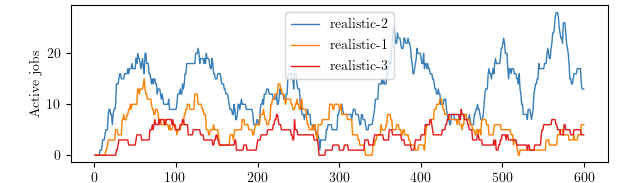
\includegraphics[width=0.9\textwidth]{../sample-output/realistic-arrivals/active-jobs.png} 
%\caption{Number of active jobs over time on small setup}
%\end{figure}
%\begin{figure}
%\centering
%\begin{minipage}{0.5\textwidth}
%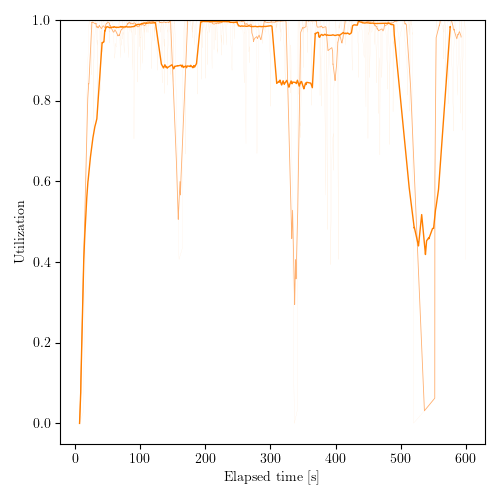
\includegraphics[width=\textwidth]{../sample-output/realistic-arrivals/utilization-rno1.png} 
%\end{minipage}%
%\begin{minipage}{0.5\textwidth}
%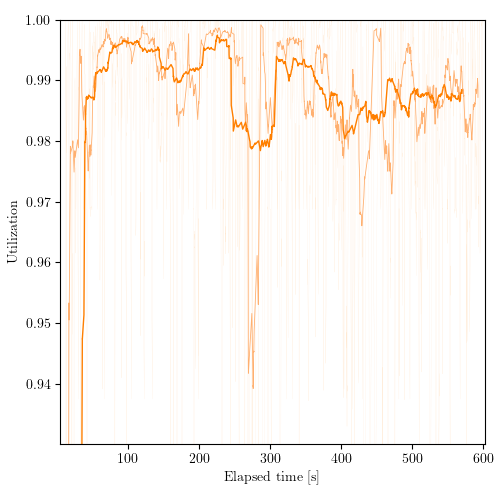
\includegraphics[width=\textwidth]{../sample-output/realistic-arrivals/utilization-rno2.png} 
%\end{minipage}%
%\caption{Utilization over time of run 1 (left) and run 2 (right)}
%\end{figure}
\begin{itemize}
 \item In terms of active jobs over time, you should be able to reproduce the same qualitative results as in our distributed setup, albeit with higher fluctuation due to fewer jobs.
 \item You should be able to observe consistent reasonably high utilization ($\approx 99\%$) at least for run 2.
 The relatively higher fluctuation on this small scale leads to lower utilization on average due to frequent re-scheduling, and, especially for low arrival rates, may lead to time intervals where not all PEs can be employed (see Section~\ref{sec:realistic-original}).
 \item The latencies reported by the respective plots for run 1 should be similarly low as in our distributed setup or lower.
 \item In terms of worker reuse, you should be able to discern improvements in terms of CCR and CS for our approach over the other two approaches.
 The absolute values for CCR and CS should be lower (since a single job experiences less relative rescheduling than in a large system) whereas we expect the values for Pr[$\cdot$] to increase more quickly than in our paper -- in our own small scale experiments, no worker was rescheduled five or more times.
\end{itemize}

\section{Troubleshooting}

The version of Mallob included in this artifact is essentially the version our originals experiments were run with, but with a few backports from our current version of Mallob to fix some bugs and errors.\footnote{We do not expect these changes to have any noticeable impact on the reported performance.}
In the following, we provide some notes on troubleshooting our software. 

\subsection{Run-Time Errors}

There is one known issue with the provided version of Mallob:
Due to a race condition, an internal assumption may fail in the solver process, which leads to this process aborting. As we have included some degree of fault-tolerance on this level, the solver process will be restarted and the scheduling of the system is not affected. This error occurs rarely (approximately once every 1\,000--10\,000 core-h), hence the impact on response times is negligible.
The error has been fixed in more recent versions of Mallob, but as our fix changes (improves) the performance of our system, we decided to rather provide the version of Mallob our experiments were conducted with.

In general, run-time errors in Mallob generate files \texttt{mallob\_thread\_trace\_*} in the base directory.
As long as a run finishes successfully, these files can be removed afterwards; however, they may provide some insights if an unexpected error occured and the entire program crashed.
In such a case, please determine whether the error occurs consistently for each run or whether a repetition of the experiment runs without errors.
(E.g., a node failure in an HPC system can lead to such a one-time error.)
If the error occurs consistently, please try to get in touch with us (see Section 4).

\subsection{Performance Problems}

If you encounter worse performance than expected in some of the experiments, please search the log files for the text ``\texttt{[WARN] Watchdog: No reset}``.
If this line occurs frequently and the indicated number of milliseconds for which no reset occurred exceeds 100\,ms, then your setup is likely to suffer from a performance problem.
Check the following points:
\begin{itemize}
\item The machine is not oversubscribed and the binding to cores is correct. In general, each MPI process should have access to $2n$ hardware threads if the option \texttt{-t=}$n$ is set.
\item The file system where the log directory resides allows for sufficiently fast logging. If possible, use a local file system or a file system with high bandwidth for your log directory. Try to reduce Mallob's verbosity (e.g., \texttt{-v=3} or \texttt{-v=2}) to probe whether this might be a problem.
\item The machine is not running demanding processes apart from Mallob.
Administration and monitoring tasks such as \texttt{ssh}, \texttt{htop}, or \texttt{tail -f} are usually fine, but computationally heavy tasks which make full use of one or multiple hardware threads are not.
\end{itemize}

If you check your local system's utilization while running Mallob, e.g., using \texttt{htop}, it should look something like this (coloring changed for better visibility):
\begin{center}
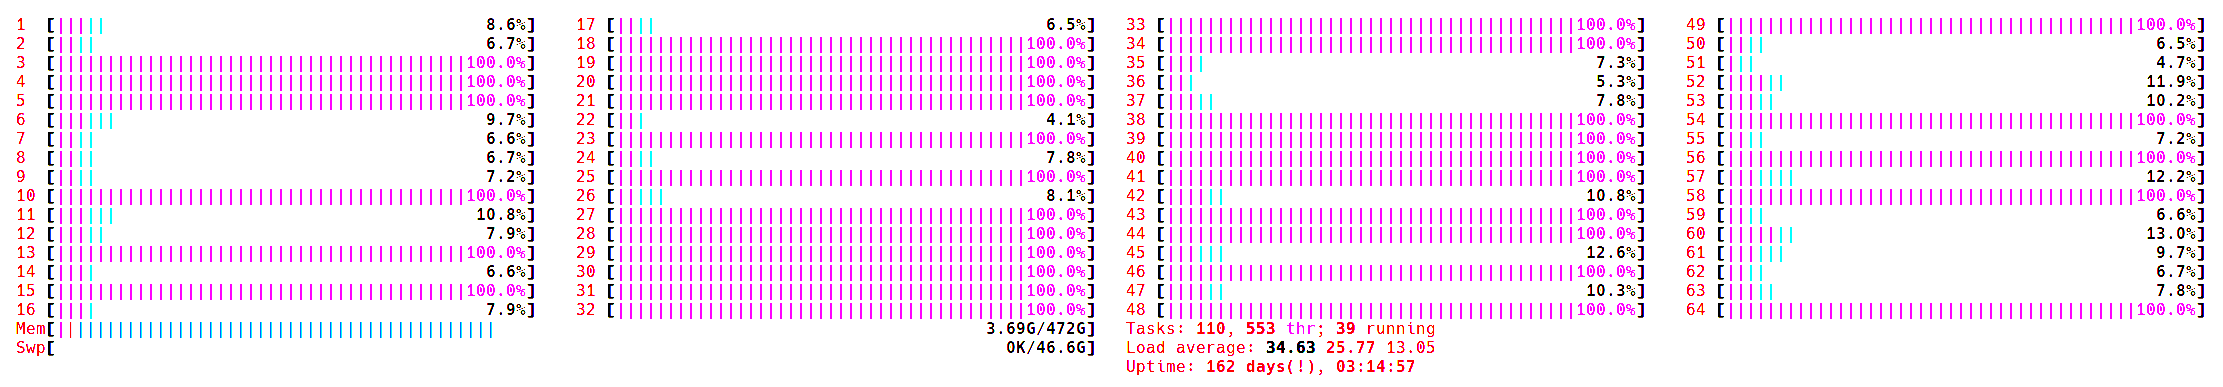
\includegraphics[width=\textwidth]{../sample-output/htop-32cores.png}
\end{center}
Note that for $1 \leq c < 32$, hardware thread $c$ is ``almost idle'' while hardware thread $c+32$ is fully utilized, or vice versa.
The only exception here is $c=32$ where both hardware threads are fully utilized; this is a ``client'' PE which currently parses a job description (SAT formula).


\section{Closing Notes}

Our software named Mallob can be accessed at \url{https://github.com/domschrei/mallob}.
Please see the license information provided there for using the different modules of Mallob.
If any questions arise, please contact \texttt{dominik.schreiber@kit.edu}.
In case this address is inactive, please try \texttt{mail@dominikschreiber.de}.
You can also submit an issue on the Github page linked above.

\subsection*{Acknowledgments}

\begin{wrapfigure}[5]{r}{0.25\textwidth}
  \vspace{-0.4cm}
  \centering
  
\includegraphics[width=\textwidth]{logo_erc_eu_tight.jpg}
\end{wrapfigure}

This project has received funding from the European Research Council (ERC) under the European Union’s Horizon 2020 research and innovation programme (grant agreement No. 882500).
The authors gratefully acknowledge the Gauss Centre for Supercomputing e.V. (www.gauss-centre.eu) for funding this project by providing computing time on the GCS Supercomputer SuperMUC-NG at Leibniz Supercomputing Centre (www.lrz.de).

% sbatch/mallob_satscheduler.sh


%
% ---- Bibliography ----
%
% BibTeX users should specify bibliography style 'splncs04'.
% References will then be sorted and formatted in the correct style.
%
%\bibliographystyle{splncs04}
%\bibliography{references_short}
%

\end{document}
